\documentclass[a4paper, 12pt]{report} % Отчёт, A4, 12 пунктов
\usepackage{fontspec} % Для выбора шрифта
\setmainfont{Times New Roman} % Устанавливаем шрифт Times New Roman
\usepackage[utf8]{inputenc} % Явно указываем кодировку текста
\usepackage[russian]{babel} % Поддержка русского языка
\usepackage{geometry} % Для настройки размера страницы и полей документа
\geometry{left=35mm, right=10mm, top=20mm, bottom=20mm}
\usepackage{setspace} % Для \onehalfspacing
\onehalfspacing % Для полуторного межстрочного интервала
\usepackage{indentfirst} 
\setlength{\parindent}{1.25cm} % Устанавливаем размер абзацного отступа
\usepackage{graphicx} % Для вставки картинок
\usepackage{titlesec} % Инструмент для настройки внешнего вида заголовков
\usepackage[titles]{tocloft} % Позволяет настраивать вид оглавления
\usepackage{caption} % Для настройки подписей к рисункам
\usepackage{listings} % Используются для вставки и подсветки исходного кода программ
\usepackage{xcolor} % Позволяет раскрашивать текст, фон страниц и таблицы

\usepackage{hyperref} % Пакет для работы со ссылками
\hypersetup{ % Настройки внешнего вида этих ссылок
	colorlinks=true,    % Делает ссылки цветными (не в рамках)
	linkcolor=black,    % Цвет ссылок на разделы/страницы (черный)
	urlcolor=blue,      % Цвет URL (синий)
}

\titleformat{\chapter}[block] % Объединяет номер главы и её название в единый текстовый блок
{\centering\bfseries}{\thechapter.}{1em}{} % Расстояние в 1 пункт (ширина буквы «M») между номером главы и её названием
\titlespacing*{\chapter}{0pt}{-30pt}{20pt} % Отступ слева, сверху, снизу

\titleformat{\section}[block] % Настройка разделов
{\bfseries}{\thesection.}{1em}{}
\titlespacing*{\section}{0pt}{20pt}{10pt} % Отступ слева, сверху, снизу

\renewcommand{\cftchapaftersnum}{.} % Добавляет точку после номера главы в оглавлении
\renewcommand{\cftsecaftersnum}{.} % Добавляет точку после номера раздела в оглавлении
\renewcommand{\cftchapfont}{\bfseries} % Названия глав - жирные
\renewcommand{\cftchappagefont}{\bfseries} % Страницы глав - жирные
\renewcommand{\cftchapleader}{\cftdotfill{\cftdotsep}} % Между названием главы и номером страницы - точки
\setlength{\cftbeforechapskip}{0.5em} % Добавляет небольшой вертикальный отступ (в пол-буквы «M») перед каждой главой

\lstdefinestyle{cppstyle}{
	language=C++,                 % Язык программирования
	basicstyle=\small\ttfamily,   % Стиль шрифта: моноширинный (печатная машинка), маленький
	keywordstyle=\color{blue},    % Цвет ключевых слов
	commentstyle=\color{green},   % Цвет комментариев
	stringstyle=\color{red},      % Цвет текста внутри кавычек
	numbers=left,                 % Нумерация строк слева
	numberstyle=\tiny\color{gray},% Стиль нумерации (очень маленькие, серого цвета)
	stepnumber=1,                 % Нумеровать каждую строку
	numbersep=5pt,                % Расстояние между номерами строк и самим кодом
	backgroundcolor=\color{white},% Цвет фона
	showspaces=false,             % Не показывать пробелы
	showstringspaces=false,       % Не показывать пробелы в строках
	showtabs=false,               % Не показывать табуляции
	frame=single,                 % Рамка вокруг кода
	rulecolor=\color{black},      % Цвет рамки
	tabsize=4,                    % Размер табуляции
	breaklines=true,              % Переносить длинные строки
	breakatwhitespace=false,      % Переносить не только по пробелам
	captionpos=t,                 % Заголовок с названием листинга будет располагаться сверху (t — top)
	keepspaces=true,			  % Сохраняем все пробелы внтури кода как есть
}

\begin{document}
	\pagenumbering{gobble} % Полностью отключаем нумерацию страниц. Это делается для того, чтобы на титульном листе не печаталась цифра «1»
	
	\begin{titlepage}
		\begin{center}
			\textbf{САНКТ-ПЕТЕРБУРГСКИЙ ПОЛИТЕХНИЧЕСКИЙ УНИВЕРСИТЕТ ПЕТРА ВЕЛИКОГО}\\
			\textbf{Институт компьютерных наук и кибербезопасности}\\
			\textbf{Высшая школа программной инженерии}\\
			\vspace{0.5cm}
			
			\begin{flushright}
				УТВЕРЖДАЮ\\
				И. О. директора ВШ ПИ\\
				П.Д. Дробинцев\\
				«\underline{\hspace{1cm}}» \underline{\hspace{3cm}}г.
			\end{flushright}
			
			\vspace{3cm}
			\textbf{ОТЧЕТ ПО ЛАБОРАТОРНОЙ РАБОТЕ №3}\\
			\vspace{0.5cm}
			\textbf{Алгоритмизация и программирование}\\
			\vspace{0.5cm}
			\textbf{Тема: Поиск автоморфных чисел на отрезке [a, b]}\\
		\end{center}
		
		\vspace{5cm}
		
		\begin{flushleft}
			Выполнил студент гр.\ 5130904/50001
			\hfill \underline{\hspace{3cm}}
			\hfill Бахуров А.С.
			
			\vspace{0.8cm}
			
			Старший преподаватель
			\hfill \underline{\hspace{3cm}}
			\hfill Самочадина Т.Н.
		\end{flushleft}
		
		\vspace{2.5cm}
		
		\begin{center}
			Санкт-Петербург\\
			2025 г.
		\end{center}
	\end{titlepage}
	
	\newpage % Переход на новую страницу
	\pagenumbering{arabic} % Нумерация - арабская
	\setcounter{page}{2} % Устанавливаем номер страницы 2
	\tableofcontents % LaTeX сам просканирует весь документ, найдет все заголовки (\chapter, \section, \subsection), соберет их названия, определит номера страниц и составит из них готовое оглавление
	
	\newpage
	
	\chapter*{Введение}
	\addcontentsline{toc}{chapter}{Введение} % Добавляем запись в оглавление
	Автоморфные числа представляют собой интересный класс чисел в теории чисел, обладающих следующим свойством:
	квадрат числа оканчивается на само это число. Классическими примерами автоморфных чисел являются 5, 6, 25, 76 и другие.
	Например, \(5^2 = 25\) (оканчивается на 5), \(25^2 = 625\) (оканчивается на 25).
	
	Целью данной лабораторной работы является разработка программы на языке C++ для поиска всех автоморфных чисел на заданном отрезке [a, b].
	Программа должна корректно обрабатывать входные данные, выполнять их валидацию в соответствии с требованиями задания и выводить
	результаты поиска в удобном для пользователя формате.
	
	Для достижения поставленной цели необходимо решить следующие задачи:
	\begin{enumerate}
		\item Реализовать алгоритм проверки числа на свойство автоморфности.
		\item Обеспечить корректный ввод границ отрезка с проверкой на числовой тип, целочисленность, положительность и корректность соотношения границ.
		\item Реализовать перебор всех чисел на заданном отрезке с выводом найденных автоморфных чисел.
		\item Разработать блок-схемы, иллюстрирующие работу основного алгоритма и функции проверки.
	\end{enumerate}
	\newpage
	
	\chapter{Основная часть}
	\section{Особенности реализации}
	Программа реализована на языке C++. Входные данные (начало отрезка \texttt{a} и конец отрезка \texttt{b}) считываются из стандартного потока ввода как числа с плавающей точкой (тип \texttt{double}) для последующей проверки на корректность согласно заданию.
	
	Алгоритм работы программы можно разделить на два основных этапа:
	\begin{enumerate} % Нумерованный список
		\item \textbf{Валидация входных данных.} Последовательно проверяются четыре условия.
		При невыполнении любого из них программа выводит соответствующее сообщение об ошибке и завершает работу.
		Для проверки на целочисленность значение переменной сравнивается с его явным приведением к целому типу \texttt{int}.
		\item \textbf{Поиск автоморфных чисел.} Если все проверки пройдены успешно, переменная \texttt{a} (начало отрезка)
		приводится к целому типу \texttt{int}. Далее в цикле \texttt{while} перебираются все целые числа от \texttt{a} до \texttt{b}
		включительно. Для каждого числа \texttt{i} вызывается функция \texttt{isAutomorphic(i)}. Если функция возвращает \texttt{true},
		число выводится на экран, а флаг \texttt{found} устанавливается в \texttt{true}.
		После завершения цикла, если флаг \texttt{found} остался равным \texttt{false}, выводится сообщение об отсутствии автоморфных чисел.
	\end{enumerate}
	
	\section{Описание алгоритма поиска автоморфных чисел}
	Автоморфным называется число, десятичная запись квадрата которого оканчивается
	десятичной записью самого числа\footnote{Определение автоморфного числа.}. % Ссылка
	Например, $25^2 = 625$, и $25$ является окончанием числа $625$.
	
	В данной работе используется классический алгоритм проверки числа \texttt{n} на свойство автоморфности:
	\begin{enumerate}
		\item Вычисляется квадрат числа: \texttt{sq = n * n}.
		\item В цикле, пока число \texttt{n} больше нуля, поразрядно сравниваются последние цифры числа \texttt{n} и его квадрата \texttt{sq}.
		\item Если на каком-либо шаге цифры не совпадают, число не является автоморфным.
		\item Если все цифры числа \texttt{n} совпали с соответствующими младшими цифрами квадрата, число считается автоморфным.
	\end{enumerate}
	
	\section{Блок-схема функции \texttt{isAutomorphic}}
	На рисунке 1 представлена блок-схема функции \texttt{isAutomorphic}.
	\begin{figure}[h!] % вставить картинку ровно в то место в тексте, где написан этот код.
		\centering
		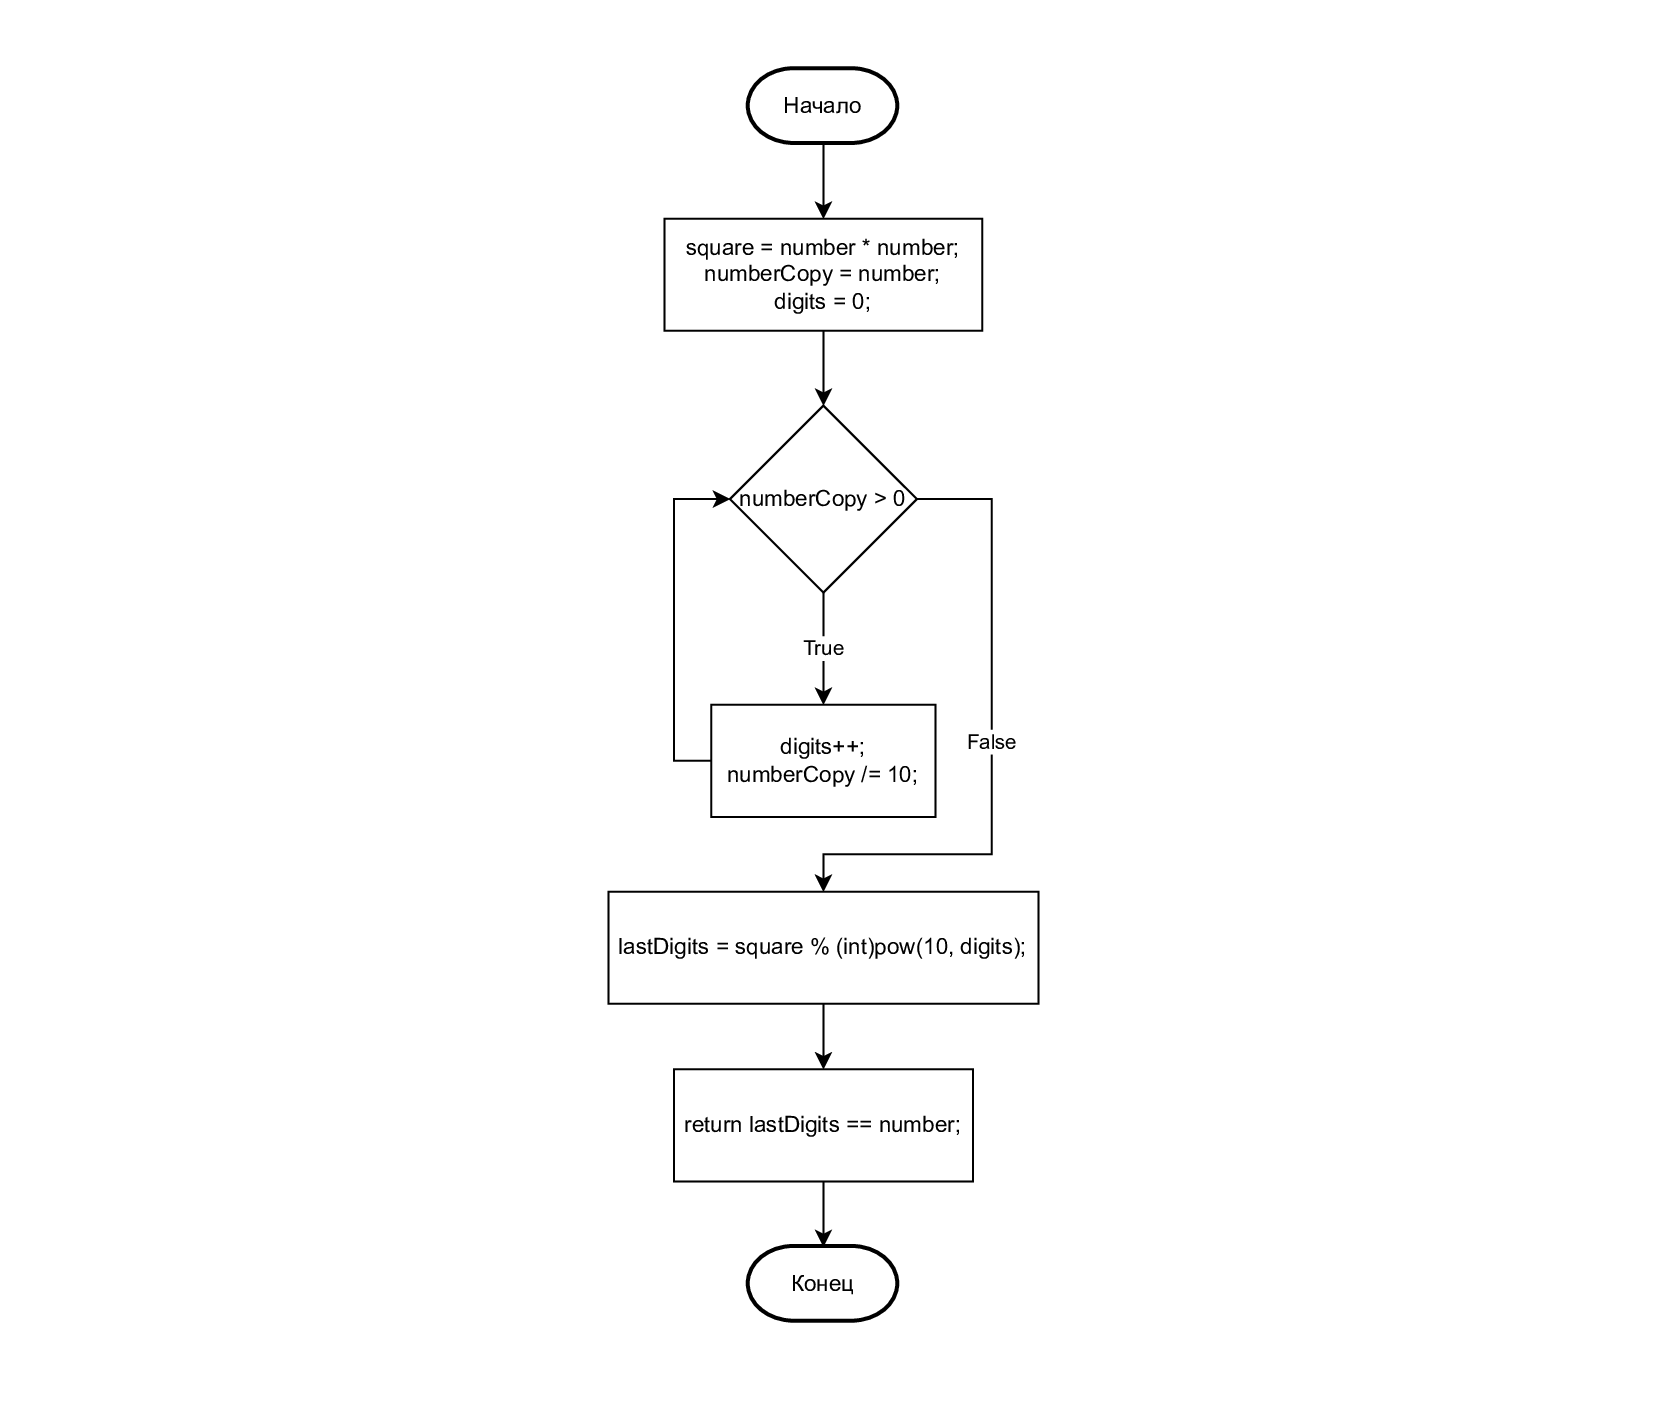
\includegraphics[width=1.0\textwidth]{АИП Блок-схема (функция).png}
		\caption*{Рисунок 1 - Блок-схема функции \texttt{isAutomorphic}}
	\end{figure}
	
	\section{Блок-схема алгоритма}
	На рисунке 2 представлена блок-схема основного алгоритма программы,
	включающая этапы валидации данных и поиска автоморфных чисел.
	
	\newpage
	
	\begin{figure}[h!]
		\centering
		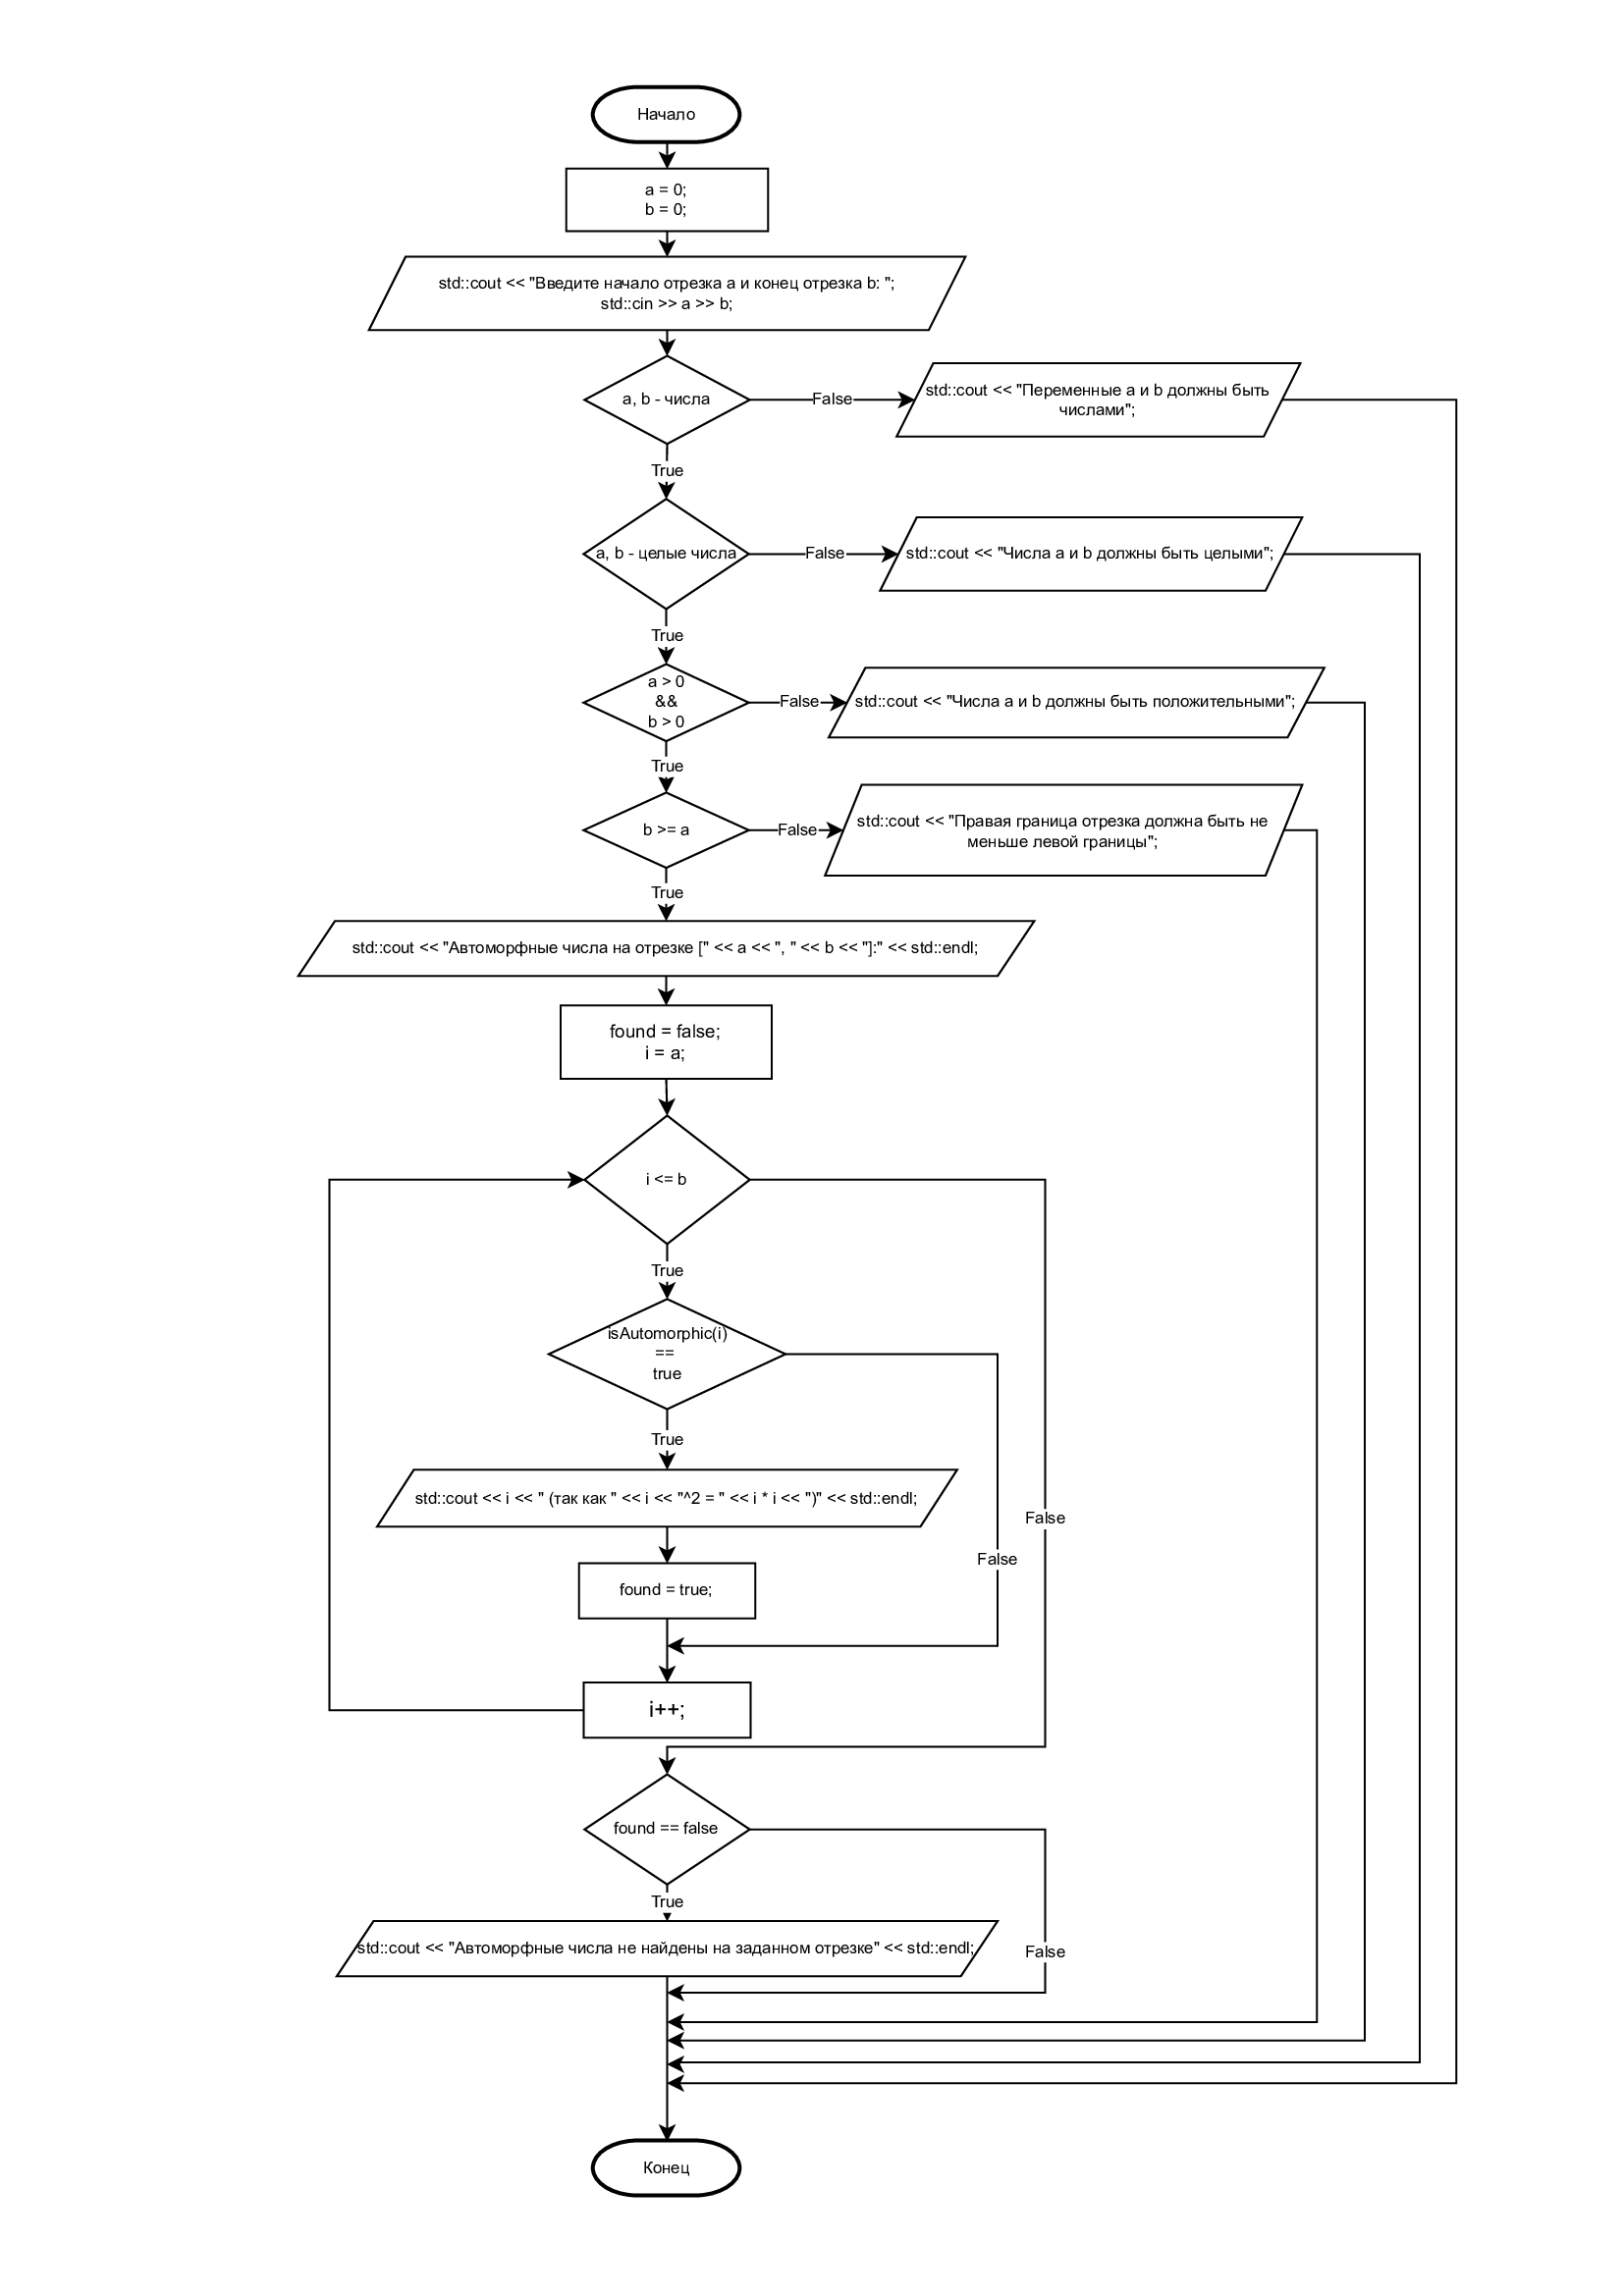
\includegraphics[width=1.0\textwidth]{АИП Блок-схема (программа).png}
		\caption*{Рисунок 2 - Блок-схема алгоритма поиска автоморфных чисел}
	\end{figure}

	\chapter*{Заключение}
	\addcontentsline{toc}{chapter}{Заключение} % Добавляем запись в оглавление
	В ходе выполнения лабораторной работы была разработана программа на языке C++ для поиска автоморфных чисел на заданном отрезке.
	Программа успешно проходит все тесты, предусмотренные в задании. Реализована полная валидация входных данных,
	что исключает возможность некорректной работы. Алгоритм поиска автоморфных чисел является эффективным и простым для понимания.
	Все требования, изложенные в задании, выполнены в полном объеме.
	
	\chapter*{Список литературы}
	\addcontentsline{toc}{chapter}{Список литературы} % Добавляем запись в оглавление
	\begin{enumerate}
		\item Страуструп Б. Язык программирования C++. Специальное издание. / Б. Страуструп. — М.: Бином, 2011. — 1136 с.
		\item Автоморфное число // Википедия. Свободная энциклопедия. — URL: \url{https://en.wikipedia.org/wiki/Automorphic_number}
		\item Шаляпин В.В. Правила оформления студенческих выпускных работ и отчетов: метод. указания / сост.: В.В. Шаляпин. - СПб.: Изд-во Политехн. ун-та, 2013. – 44с.
	\end{enumerate}
	
	\newpage
	
	\addcontentsline{toc}{chapter}{Приложение А.}
	\begin{flushright}
		\textbf{Приложение А}
	\end{flushright}
	\begin{lstlisting}[style=cppstyle]
int main()  
{  
	double a = 0; 
	double b = 0; 
	std::cout << "Enter the start point a and the end point b: "; 
	std::cin >> a >> b; 
	if (std::cin.fail()) { 
		std::cout << "Variables a and b must be numbers"; 
	} 
	else if (a != static_cast<int>(a) || b != static_cast<int>(b)) { 
		std::cout << "The numbers a and b must be integers"; 
	} 
	else if (a <= 0 || b <= 0) { 
		std::cout << "The numbers a and b must be positive"; 
	} 
	else if (a > b) { 
		std::cout << "The right boundary of the segment must be at least as large as the left boundary"; 
	} 
	else { 
		std::cout << "Automorphic numbers on a segment [" << a << ", " << b << "]:" << std::endl; 
		bool found = false; 
		int i = a; 
		while (i <= b) { 
			if (isAutomorphic(i) == true) { 
				std::cout << i << " (because " << i << "^2 = " << i * i << ")" 
				<< std::endl; 
				found = true; 
			} 
			i++; 
		} 
		if (found == false) { 
			std::cout << "No automorphic numbers are found in the given interval" << std::endl; 
		} 
	} 
	return 0; 
}
	\end{lstlisting}
\end{document}